\documentclass[12pt]{article}
\usepackage{amsfonts, amssymb, amsmath, amsthm}
\usepackage[margin=1in]{geometry}
\usepackage{tikz}

\title{Explainer: Problem 6 (Rudin 7.14) --- The Schoenberg Space-Filling Curve}
\author{}
\date{}

\begin{document}
\maketitle

\section*{What's going on?}
We're constructing a \textbf{continuous} curve $\Phi : [0,1] \to \mathbb{R}^2$ that fills the entire unit square $[0,1]^2$. This is deeply counterintuitive --- a one-dimensional curve covers a two-dimensional region!

The construction uses a helper function $f$ and the Cantor set.

\section*{The helper function $f$}

$f$ is periodic with period 2, and on $[0,1]$:

\begin{center}
\begin{tikzpicture}[scale=3]
    \draw[->] (-0.1,0) -- (2.3,0) node[right] {$t$};
    \draw[->] (0,-0.1) -- (0,1.2) node[above] {$f(t)$};

    % [0, 1/3]: f=0
    \draw[thick, blue] (0,0) -- (0.333,0);
    % [1/3, 2/3]: transition
    \draw[thick, blue, dashed] (0.333,0) -- (0.667,1);
    % [2/3, 1]: f=1
    \draw[thick, blue] (0.667,1) -- (1,1);
    % [1, 4/3]: f=1
    \draw[thick, blue] (1,1) -- (1.333,1);
    % [4/3, 5/3]: transition
    \draw[thick, blue, dashed] (1.333,1) -- (1.667,0);
    % [5/3, 2]: f=0
    \draw[thick, blue] (1.667,0) -- (2,0);

    \node[below] at (0.333,0) {\tiny $\frac{1}{3}$};
    \node[below] at (0.667,0) {\tiny $\frac{2}{3}$};
    \node[below] at (1,0) {\tiny $1$};
    \node[below] at (1.333,0) {\tiny $\frac{4}{3}$};
    \node[below] at (1.667,0) {\tiny $\frac{5}{3}$};
    \node[below] at (2,0) {\tiny $2$};
    \node[left] at (0,1) {\tiny $1$};
\end{tikzpicture}
\end{center}

The key property: $f$ is $0$ on $[0, 1/3]$ and $1$ on $[2/3, 1]$. It transitions smoothly in between. By periodicity, $f$ reads off the ``digits'' of a base-3 expansion.

\section*{The curve $\Phi(t) = (x(t), y(t))$}

$$
x(t) = \sum_{n=1}^{\infty} 2^{-n} f(3^{2n-1} t), \qquad y(t) = \sum_{n=1}^{\infty} 2^{-n} f(3^{2n} t).
$$

The idea: $3^k t$ ``shifts'' the base-3 expansion of $t$ by $k$ digits. Applying $f$ reads off whether that digit is $0$ or $2$ (the Cantor set digits). The $2^{-n}$ weighting assembles these into a binary expansion.

\section*{Continuity of $\Phi$}

Each term $2^{-n} f(3^k t)$ is continuous (it's a continuous function composed and scaled). The series converges uniformly by the Weierstrass $M$-test ($|2^{-n} f(3^k t)| \leq 2^{-n}$ and $\sum 2^{-n} < \infty$). By Theorem 7.12, $x(t)$ and $y(t)$ are continuous, hence $\Phi$ is continuous.

\section*{Surjectivity: why $\Phi$ hits every point in $[0,1]^2$}

Pick any $(x_0, y_0) \in [0,1]^2$. Write their binary expansions:
$$
x_0 = \sum_{n=1}^{\infty} 2^{-n} a_{2n-1}, \qquad y_0 = \sum_{n=1}^{\infty} 2^{-n} a_{2n},
$$
where each $a_i \in \{0, 1\}$. Now \textbf{interleave} these bits into a base-3 number:
$$
t_0 = \sum_{i=1}^{\infty} \frac{2a_i}{3^{i+1}}.
$$

\begin{center}
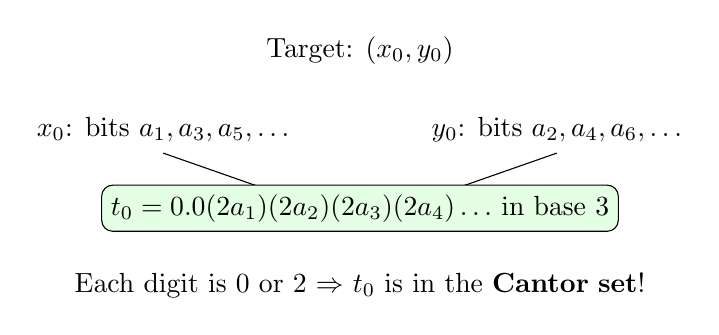
\begin{tikzpicture}[>=stealth]
    \node at (0,2) {Target: $(x_0, y_0)$};
    \node at (-2.5, 1) {$x_0$: bits $a_1, a_3, a_5, \ldots$};
    \node at (2.5, 1) {$y_0$: bits $a_2, a_4, a_6, \ldots$};
    \draw[->] (-2.5, 0.7) -- (-0.5, 0);
    \draw[->] (2.5, 0.7) -- (0.5, 0);
    \node[draw, rounded corners, fill=green!10] at (0, 0) {$t_0 = 0.0(2a_1)(2a_2)(2a_3)(2a_4)\ldots$ in base 3};
    \node[below, text width=8cm, align=center] at (0, -0.7) {Each digit is $0$ or $2$ $\Rightarrow$ $t_0$ is in the \textbf{Cantor set}!};
\end{tikzpicture}
\end{center}

Since each $2a_i \in \{0, 2\}$, the number $t_0$ has only digits $0$ and $2$ in base 3 --- it's in the Cantor set. One then checks $f(3^k t_0) = a_k$, so $\Phi(t_0) = (x_0, y_0)$.

\section*{Proof outline}
\begin{enumerate}
    \item \textbf{Continuity:} Weierstrass $M$-test with $M_n = 2^{-n}$.
    \item \textbf{Surjectivity:} Given $(x_0, y_0)$, construct $t_0$ in the Cantor set by interleaving binary digits. Verify $f(3^k t_0) = a_k$ using $f$'s definition on $[0,1/3]$ and $[2/3, 1]$.
    \item \textbf{Cantor set:} $t_0$ has only digits $0, 2$ in base 3, so $t_0 \in C$.
\end{enumerate}

\end{document}